\documentclass{beamer}
\usepackage{../common_slides}
\usepackage{tikz}
\usepackage{tikz-qtree}
\usepackage{pdfpages}

\usetikzlibrary{matrix}
% \usepackage{enumitem}

\title{Sequence Models 4}
\date{}
\author{CS 287}

\def\Lattice{
    \matrix (network)
    [matrix of nodes,
    nodes in empty cells,
    ampersand replacement=\&,
    column sep={1cm},
    row sep={0.1cm},
    nodes={outer sep=0pt,circle,minimum size=0.5cm, minimum width=1.3cm,draw, rectangle} ]
    {
     O \& O \& O \& O \& O\\
     I-PER \& I-PER \& I-PER \& I-PER \& I-PER \\ 
     I-ORG \& I-ORG \& I-ORG \& I-ORG \& I-ORG \\ 
     I-LOC \& I-LOC \& I-LOC \& I-LOC \& I-LOC \\ 
     |[draw=none]| \\
     |[draw=none]| Mayor \& |[draw=none]| DeBlasio \& |[draw=none]| from \& |[draw=none]| New  \& |[draw=none]| York  \\  
};
}

\def\LatticeB{
    \matrix (network)
    [matrix of nodes,
    nodes in empty cells,
    ampersand replacement=\&,
    column sep={1cm},
    row sep={0.1cm},
    nodes={outer sep=0pt,circle,minimum size=0.5cm, minimum width=1.3cm,draw, rectangle} ]
    {
     O \& O \& O \& O \& O\\
     I-PER \& I-PER \& I-PER \& I-PER \& I-PER \\ 
     I-ORG \& I-ORG \& I-ORG \& I-ORG \& I-ORG \\ 
     I-LOC \& I-LOC \& I-LOC \& I-LOC \& I-LOC \\ 
     |[draw=none]| \\
     |[draw=none]| The \& |[draw=none]| United \& |[draw=none]| Nations \& |[draw=none]| will  \& |[draw=none]| meet  \\  
};
}


\begin{document}
\begin{frame}
  \titlepage
\end{frame}

\begin{frame}{Review: Backward Viterbi}
  % \begin{itemize}
  % \item Same speed, same results.
  % \item Similar inductive rule applies.
  % \item Construct sequences starting at the end. 
  % \end{itemize}

  \begin{algorithmic}
    \Procedure{BackwardViterbi}{}
    \State{$\pi \in \reals^{ (n+1) \times \mcC}$ initialized to $-\infty$ }
    \State{$\pi[n+1, \langle /s \rangle] = 0$}
    \For{$i = n$ to $1$ }
    \For{$c_{i} \in \mcC$}
    \State{$\pi[i, c_i] = \max_{c'_{i+1}} 
     \pi[i+1, c'_{i+1}] + \log \hat{y}(c_{i})_{c'_{i+1}}        
       $}
    \EndFor{}
    \EndFor{}
    \State{\Return{$\max_{c_1\in\mcC} \pi[1, c_1]$}}
    \EndProcedure{}
  \end{algorithmic}
\end{frame}

\begin{frame}{Review: Edge Marginal}
  \begin{center}
   
  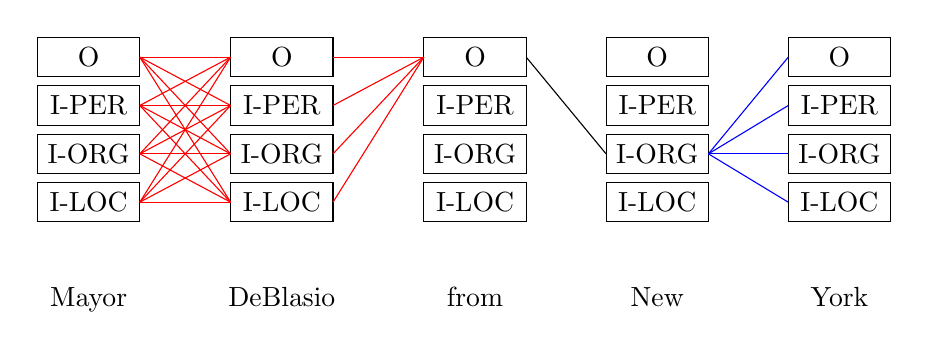
\begin{tikzpicture}
    \Lattice

    \draw[blue] (network-3-4.east) -- (network-1-5.west);
    \draw[blue] (network-3-4.east) -- (network-2-5.west); 
    \draw[blue] (network-3-4.east) -- (network-3-5.west);
    \draw[blue] (network-3-4.east) -- (network-4-5.west);
    \draw[black] (network-1-3.east) -- (network-3-4.west);

    \draw[red] (network-1-3.west) -- (network-1-2.east);
    \draw[red] (network-1-3.west) -- (network-2-2.east); 
    \draw[red] (network-1-3.west) -- (network-3-2.east);
    \draw[red] (network-1-3.west) -- (network-4-2.east);

    \foreach \i in {1,...,4} {
    \foreach \j in {1,...,4} {
    \draw[red] (network-\i-1.east) -- (network-\j-2.west);
    % \draw[red] (network-\i-2.east) -- (network-\j-3.west);
    % \draw[red] (network-\i-3.east) -- (network-\j-4.west);
    % \draw[blue] (network-\i-4.east) -- (network-\j-5.west);
    } }

  \end{tikzpicture}
  \end{center}  
\end{frame}


\begin{frame}{Review:  Marginals}
  Assume we \textbf{are not} given $c_{1:i-1}$ and $c_{i+1:n}$.
  \air 

  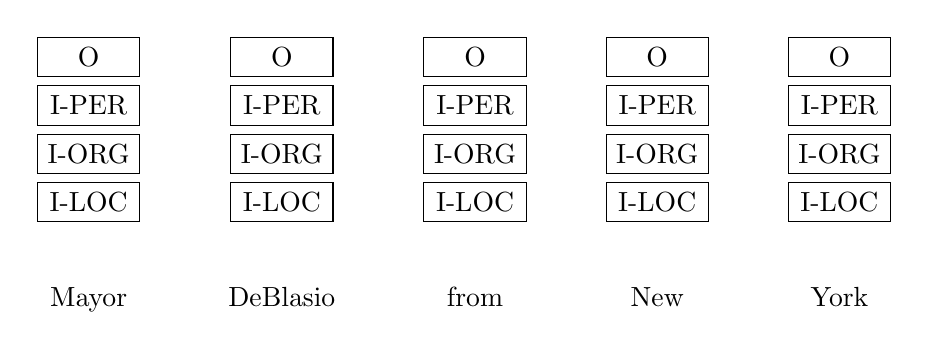
\begin{tikzpicture}
    \Lattice
    % \draw[red] (network-2-1.north west) rectangle  (network-2-1.south east);
    % \draw[red] (network-2-2.north west) rectangle  (network-2-2.south east);
    % \draw[red] (network-4-4.north west) rectangle  (network-4-4.south east);
    % \draw[red] (network-4-5.north west) rectangle  (network-4-5.south east);
  \end{tikzpicture}

  What is the best completed sequence, i.e. 
  \begin{eqnarray*}
    p(\boldy_i = \delta(c_i)| \boldx)
  \end{eqnarray*}
\end{frame}


\begin{frame}{Answer: Marginalization}
  \begin{itemize}
  \item Similar idea. Score involving $c_i$ are local ($i-1$ and $i+1$).
    \air 


    \begin{eqnarray*}
    p(\boldy_i = \delta(c'_i)| \boldx) &=& \sum_{c_{1:i-1}:c_{i+1:n}} p(\bold{y}_i = \delta(c'_i),  \boldy_{1:i-1,i+1:n}| \boldx ) \\ 
                                       &=& \sum_{c_{1:i-1}} p(\boldy_{1:i-1}|\boldx) p(\bold{y}_i = \delta(c'_i)|  \boldy_{i-1},  \boldx ) \\
                                       &\times&  \sum_{c_{i+1:n}} p(\bold{y}_{i+1}| \boldy_{i} = , \boldx) p(\bold{y}_{i+1:n}|\boldx) \\       \pause
                                       &= & \sum_{c_{1:i-1}} \hat{y}(c_{i-1})_{c'_{i}}  \prod_{j=1}^{i-1} \hat{y}(c_{j-1})_{c_{j}}  \\
                                       &\times& \sum_{c_{i+1:n}}  \hat{y}(c'_{i})_{c_{i+1}} \prod_{j=i+1}^n   \hat{y}(c_{j})_{c_{j+1}} \\      
    \end{eqnarray*}
    \air 
  \end{itemize}
\end{frame}

\begin{frame}{Review: Edge Marginals}
  \begin{eqnarray*}
    && \hat{y}(c'_{i})_{c'_{i+1}} \times \sum_{c_{1:i-1}} \hat{y}(c_{i-1})_{c'_{i}}  \prod_{j=1}^{i-1} \hat{y}(c_{j-1})_{c_{j}}  \\
     &\times& \sum_{c_{i+2:n}}  \hat{y}(c'_{i+1})_{c_{i+1}} \prod_{j=i+1}^n   \hat{y}(c_{j})_{c_{j+1}} \\          
  \end{eqnarray*}

  % \[ \argmax_{c_i, c_{i+1}} \max_{c_{1:i-1}:c_{i+2:n}} f(\boldx, c_{1:n}) \] 
  \begin{itemize}
  \item Compute $\alpha$ using Forward
    \air 

  \item Compute $\beta$ using Backward 
    \air

  \item Multiply in the edge 
    \[ \hat{y}(c'_{i})_{c'_{i+1}} \times \alpha[i, c'_i] \times \beta[i+1, c'_{i+1}] \] 
  \end{itemize}
\end{frame}


\begin{frame}{Quiz}
  Last class we looked at discriminative sequence models 
  $p(\boldy | \boldx)$. Consider now a generative model (such as 
  an HMM), where we model $p(\boldy, \boldx)$. 

  Unlike a discriminative model, we can use to compute the probability of a specific $\boldx$ by marginalizing out $\boldy$, $p(\boldx) = \sum_{c_{1:n}} p(\boldy = \delta(c_{1:n}), \boldx)$. 


  \begin{itemize}
  \item How do you compute this?
    \air
  \item What value should this same algorithm give you in the discriminative case?
  \end{itemize}
\end{frame}

\begin{frame}{Answer}
  \[p(\boldx) = \sum_{c_{1:n}} p(\boldy = \delta(c_{1:n}), \boldx)\]

  Return value here. 

  \begin{algorithmic}
    \Procedure{Forward}{}
    \State{$\alpha \in \reals^{\{0,\ldots, n\} \times \mcC}$ initialized to $-\infty$ }
    \State{$\alpha[0, \langle s \rangle] = 0$}
    \For{$i = 1$ to $n$ }
    \For{$c_{i} \in \mcC$}
    \State{$\alpha[i, c_i] = \sum_{c_{i-1}} 
     \alpha[i-1, c_{i-1}] * \hat{y}(c_{i-1})_{c_i}        
       $}
    \EndFor{}
    \EndFor{}
    \State{\Return{$\sum_{c_n\in\mcC} \alpha[n, c_n]$}}
    \EndProcedure{}
  \end{algorithmic}

  \begin{itemize}
  \item In the discriminative case, sums to $1$ (nice unit test)
  \end{itemize}
\end{frame}


% \begin{frame}{Today's Lecture}
%   \begin{itemize}
%   \item Sequence 
%   \end{itemize}
% \end{frame}

\begin{frame}{Sequence Models Zoology}
  \begin{itemize}

  \item Generative versus Discriminative Model
    \air 
  \item Local versus Sequence Prediction
    \air 
  \item Probabilistic versus Non-probabilistic Objective
    \air 
  \item Markov versus Non-Markov Model
    \air 
  \item Linear versus Non-Linear Model
  \end{itemize}
\end{frame}

\begin{frame}{Model Choices}
  Examples of discriminative sequence model with local prediction
  \air 

  \begin{center}
    \begin{tabular}{llcc}
      \toprule
       && Markov ($\hat{\boldy}(c_{i-1})$) & Non-Markov ($\hat{\boldy}(c_1, \ldots, c_{i-1})$) \\ 
      \midrule
      Linear &&  MEMM &  LR with global features  \\ 
      Non-Linear (NN) && NNLM &  RNN (transducer) \\ 
      \bottomrule
    \end{tabular}
  \end{center}
\end{frame}




\begin{frame}{Model Choices}
  Examples of linear discriminative models   
  \[p(\boldy | \boldx)\] 
  \begin{center}
    \begin{tabular}{llcc}
      \toprule
      &&  Local & Sequence \\ 
      \midrule
      Probabilistic  && MEMM &  CRF (new) \\ 
      Non-Probabilistic && N/A & Structured Perceptron/SVM \\ 
      \bottomrule
    \end{tabular}
  \end{center}
\end{frame}

\begin{frame}{Model Choices}
  Examples of linear, generative probabilistic models
  \air 
  \[p(\boldx, \boldy)\] 

  \begin{center}
    \begin{tabular}{llcc}
      \toprule
       && Local & Sequence \\ 
      \midrule
      Linear &&  HMM &  MRF (new)  \\ 
      \bottomrule
    \end{tabular}
  \end{center}
\end{frame}

\section{Local Prediction in Sequence Models }

\begin{frame}{Benefits of Local Prediction Markov Models}
  \begin{itemize}
  \item Relatively easy to train (multi-class)
    \air 

    
  \item Particularly convenient to use with NN $(\hat{\boldy}(c_i))$
    \air 

  \item Can use same decoding algorithms (Viterbi, forward, backward)
  \end{itemize}
\end{frame}

\begin{frame}{Review: Entropy of a Distribution}
  \begin{itemize}

    \air 
  \item Recall: entropy of distribution
    \[H(\boldy) = - \sum_{i} p(\boldy_i) \log p(\boldy_i) \]
    
  \end{itemize}
  \begin{center}
    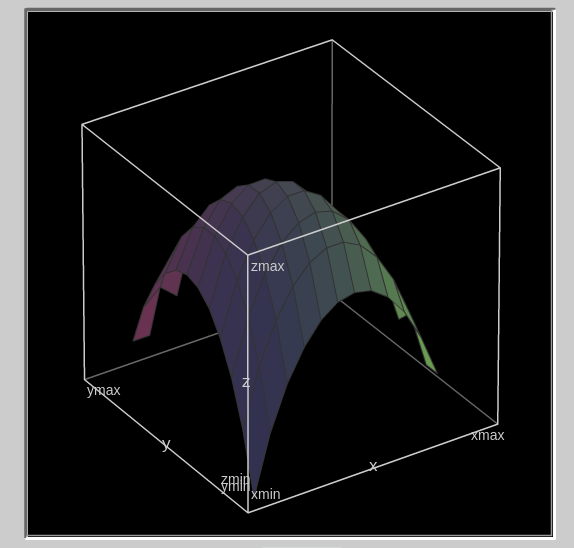
\includegraphics[width=6cm]{entropy}
  \end{center}
\end{frame}


\begin{frame}{Issue: Label Bias (Bottou, 1991)}
  \begin{itemize}
   \item Local normalization can lead to pathological sequence
    scores $f$.
    \air 

  \item Issue: low-entropy (spiky) transitions $\boldy(c_{i-1})$
    \air 

  \item Can cause the model to ignore input $\boldx_i$
  \end{itemize}
\end{frame}

% \begin{frame}{Low-Entropy Scenarios}
%   \begin{itemize}
%   \item Consider the named-entity recognition case
%       \end{itemize}
% \end{frame}

\begin{frame}{Label Bias Example 1}
  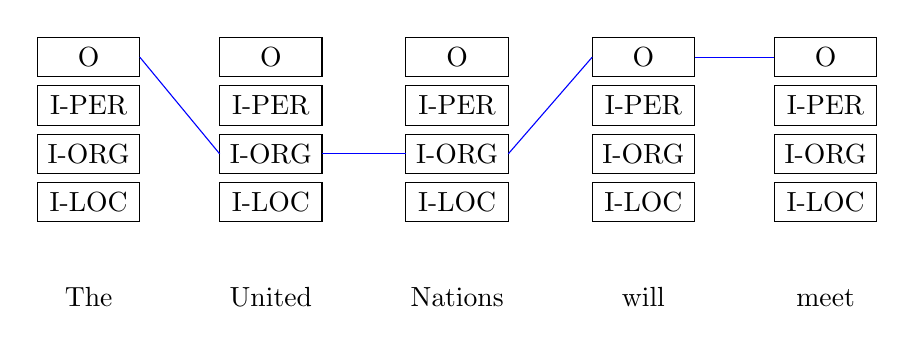
\begin{tikzpicture}
    \LatticeB
    \draw[blue] (network-1-1.east) --  (network-3-2.west);
    \draw[blue] (network-3-2.east) --  (network-3-3.west);
    \draw[blue] (network-3-3.east) --  (network-1-4.west);
    \draw[blue] (network-1-4.east) --  (network-1-5.west);
  \end{tikzpicture}
  \begin{itemize}
  \item Correct example, should have a high score.
    \[ f(\boldx, c_{1,n}) \] 
  \end{itemize}
\end{frame}


\begin{frame}{Label Bias Example 2}
  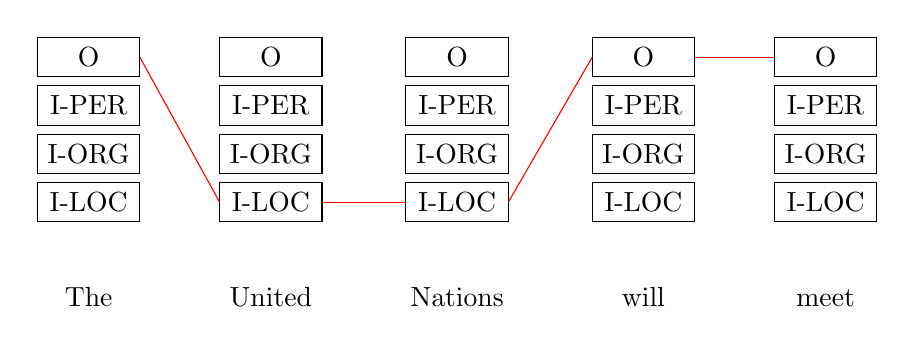
\begin{tikzpicture}
    \LatticeB
    \draw[red] (network-1-1.east) --  (network-4-2.west);
    \draw[red] (network-4-2.east) --  (network-4-3.west);
    \draw[red] (network-4-3.east) --  (network-1-4.west);
    \draw[red] (network-1-4.east) --  (network-1-5.west);
  \end{tikzpicture}
  \begin{itemize}
  \item Very incorrect example, should have a low score.
    \[ f(\boldx, c_{1,n}) \] 
  \end{itemize}
\end{frame}


\begin{frame}{Label Bias Example 3}
  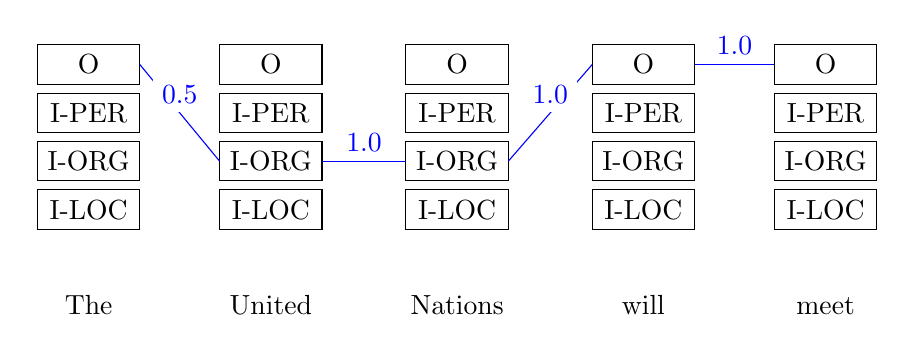
\begin{tikzpicture}
    \LatticeB
    \draw[blue] (network-1-1.east) -- node[above,fill=white]{0.5}  (network-3-2.west);
    \draw[blue] (network-3-2.east) -- node[above,fill=white]{1.0} (network-3-3.west);
    \draw[blue] (network-3-3.east) -- node[above,fill=white]{1.0} (network-1-4.west);
    \draw[blue] (network-1-4.east) -- node[above,fill=white]{1.0} (network-1-5.west);
  \end{tikzpicture}
  \begin{itemize}
  \item Correct example, should have a high score.
    \[ f(\boldx, c_{1,n}) = \log(0.5) + \log(1.0) + \log(1.0) + \log(1.0) \] 
  \end{itemize}
\end{frame}


\begin{frame}{Label Bias Example 4}
  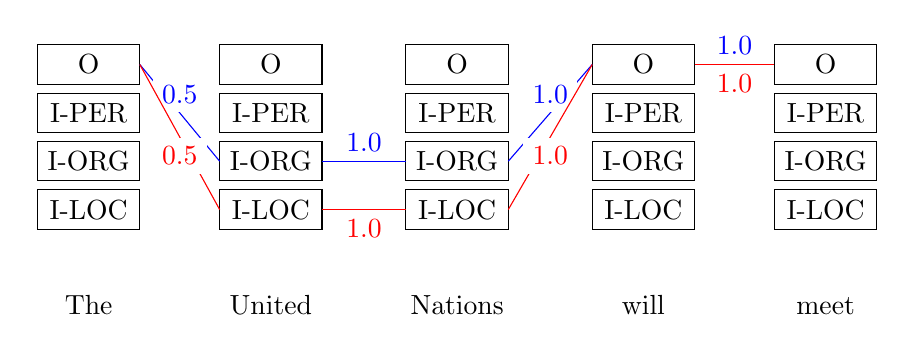
\begin{tikzpicture}
    \LatticeB
    \draw[blue] (network-1-1.east) -- node[above,fill=white]{0.5}  (network-3-2.west);
    \draw[blue] (network-3-2.east) -- node[above,fill=white]{1.0} (network-3-3.west);
    \draw[blue] (network-3-3.east) -- node[above,fill=white]{1.0} (network-1-4.west);
    \draw[blue] (network-1-4.east) -- node[above,fill=white]{1.0} (network-1-5.west);
    \draw[red] (network-1-1.east) -- node[below,fill=white]{0.5}  (network-4-2.west);
    \draw[red] (network-4-2.east) -- node[below,fill=white]{1.0}  (network-4-3.west);
    \draw[red] (network-4-3.east) -- node[below,fill=white]{1.0}  (network-1-4.west);
    \draw[red] (network-1-4.east) --node[below,fill=white]{1.0}  (network-1-5.west);
  \end{tikzpicture}
  \begin{itemize}
  \item Correct example, should have a high score.
    \[ f(\boldx, c_{1,n}) = \log(0.5) + \log(1.0) + \log(1.0) + \log(1.0) \] 
  \item Very incorrect example, should have a low score.
    \[ f(\boldx, c_{1,n}) = \log(0.5) + \log(1.0) + \log(1.0) + \log(1.0)\] 

  \end{itemize}
\end{frame}

\begin{frame}{Issue: Local Normalization}
  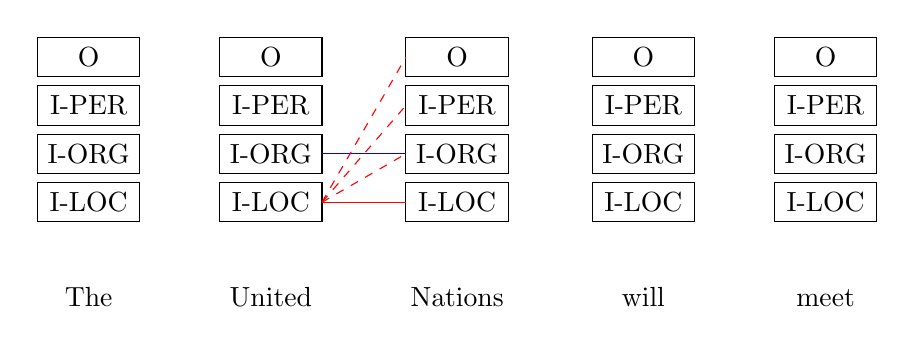
\begin{tikzpicture}
    \LatticeB
    % \draw[blue] (network-1-1.east) -- node[above,fill=white]{0.5}  (network-3-2.west);
    \draw[blue] (network-3-2.east) --  (network-3-3.west);
    % \draw[blue] (network-3-3.east) -- node[above,fill=white]{1.0} (network-1-4.west);
    % \draw[blue] (network-1-4.east) -- node[above,fill=white]{1.0} (network-1-5.west);
    % \draw[red] (network-1-1.east) -- node[below,fill=white]{0.5}  (network-4-2.west);
    \draw[red] (network-4-2.east) -- (network-4-3.west);
    \draw[red,dashed] (network-4-2.east) --   (network-1-3.west);
    \draw[red,dashed] (network-4-2.east) --   (network-3-3.west);
    \draw[red,dashed] (network-4-2.east) --   (network-2-3.west);
    % \draw[red] (network-4-3.east) -- node[below,fill=white]{1.0}  (network-1-4.west);
    % \draw[red] (network-1-4.east) --node[below,fill=white]{1.0}  (network-1-5.west);
  \end{tikzpicture}
  \begin{itemize}
  \item At I-LOC, we only have 4 choices, 2 of which have 0 prob. 
  \item Of the option only I-LOC makes sense (definitely not O). 
  \item Local model, cannot report current path is \alert{wrong}
  \item Effectively ignores input \textit{Nations}
  \end{itemize}
\end{frame}


\begin{frame}{Further Issues}
  \begin{itemize}
  \item Note: this is a modeling issue, not a search issue. 
    \air 
  \item i.e. failure even with exact search.
    \air 

  \item Related issue: Exposure Bias. 
    \air 
  \item Training never condition on incorrect decisions.
  \end{itemize}
\end{frame}

\section{Conditional Random Fields}

\begin{frame}{Issues with Multiclass for Sequences (3rd time!) }
  \begin{itemize}
  \item Say there are $\mcC$ tags and sequence length is $n$
    \air 

  \item There are $\dout = O(\mcC^n)$ sequences! 
    \air 
  \item Just naively computing the softmax is exponential in length. 
    \air 

  \item Even if you could compute the softmax, $\boldW \in \reals^{\din \times \dout}$ would 
    be impossible to train.
  \end{itemize}
\end{frame}

\begin{frame}{(Linear Chain) Conditional Random Field (Lafferty et al, 2001)}
  \begin{itemize}
  \item Model consists of unnormalized weights 

    \[\log \hat{\boldy}(c_{i-1})_{c_i} = feat(\boldx, c_{i-1}) \boldW + \boldb\]
    
  \item Out of log space, 

    \[ \hat{\boldy}(c_{i-1})_{c_i} = \exp(feat(\boldx, c_{i-1}) \boldW + \boldb)\]

    

  \item Score of the sequence, (same as last few classes)
    
    \[ f(\boldx, c_{1:n}) = \sum_{i=1}^n \log \hat{y}(c_{i-1})_{c_{i}} \] 
    % \[ p(\boldy  | \boldx ) =  \softmax\ \mathrm { over\ all\ sequences}    \] 

  \item Objective is based on global NLL of this sequence distribution
    \[\boldz_{c_{1:n}} =  f(\boldx, c_{1:n})    \] 

  \end{itemize}
\end{frame}

\begin{frame}{Distribution over Sequences}

  \begin{itemize}
  \item 
  How do we compute the probability of sequences?

  \item Softmax over scores,
    \[ p(\boldy = \delta(c_{1:n}) | \boldx ) =  \softmax(f(\boldx, c_{1:n}))    \] 

  \item What does this look like?
  \begin{eqnarray*}
    p(\boldy=\delta(c_{1:n}) | \boldx ) &=& \displaystyle \frac{\displaystyle \exp \left( \sum_{i=1}^n \log \hat{y}(c_{i-1})_{c_{i}}\right) }{\displaystyle \sum_{c'_{1:n}} \exp\left(\sum_{i=1}^n \log \hat{y}(c'_{i-1})_{c'_{i}} \right) }  \\       
    &=& \frac{\displaystyle \prod_{i=1}^n \hat{\boldy}(c_{i-1})_{c_i}} { \displaystyle \sum_{c'_{1:n}} \prod_{i=1}^n \hat{\boldy}(c'_{i-1})_{c'_i} }
  \end{eqnarray*}
\end{itemize}
 \end{frame}


 \begin{frame}{Computing the Softmax}
   Want to compute:
   \[ p(\boldy=\delta(c_{1:n}) | \boldx) = \frac{\displaystyle \prod_{i=1}^n \hat{\boldy}(c_{i-1})_{c_i}} {\displaystyle  \sum_{c'_{1:n}} \prod_{i=1}^n \hat{\boldy}(c'_{i-1})_{c'_i} }\] 

   \begin{itemize}
   \item $\displaystyle \prod_{i=1}^n \hat{\boldy}(c_{i-1})_{c_i}$; easy to compute
     \air 
   \item $\displaystyle \sum_{c'_{1:n}} \prod_{i=1}^n \hat{\boldy}(c'_{i-1})_{c'_i}$; can use forward algorithm.
   \end{itemize}

   Softmax goes from $O(|\mcC|^n)$ to $O(|\mcC|^2)$.  
 \end{frame}

\begin{frame}{Forward Algorithm}
  \begin{algorithmic}
    \Procedure{Forward}{}
    \State{$\alpha \in \reals^{\{0,\ldots, n\} \times \mcC}$  }
    \State{$\alpha[0, \langle s \rangle] = 1$}
    \For{$i = 1$ to $n$ }
    \For{$c_{i} \in \mcC$}
    \State{$\alpha[i, c_i] = \sum_{c_{i-1}} 
     \alpha[i-1, c_{i-1}] \times \hat{y}(c_{i-1})_{c_i}        
       $}
    \EndFor{}
    \EndFor{}
    \State{\Return{$\alpha$}}
    \EndProcedure{}
  \end{algorithmic}
\end{frame}


 \begin{frame}{Computing Marginals}
   Want to compute:
   \begin{eqnarray*}
    p(\boldy_i =\delta_{c_i} | \boldx) &=& \sum_{c_{1:i-1}, c_{i+1:n}} p(\boldy | \boldx)  \\
     &=& \frac{\displaystyle \left(\sum_{c_{1:i-1}} \prod_{j=1}^{i-1} \boldy(c_{j-1})_{c_j} \right) \left(\sum_{c_{i+1:n}} \prod_{j=i+1}^{n} \boldy(c_{j-1})_{c_j} \right)   } {\displaystyle \sum_{c'_{1:n}} \prod_{i=1}^n \hat{\boldy}(c'_{i-1})_{c'_i}}        
   \end{eqnarray*}


   \begin{itemize}
   \item $\displaystyle \sum_{c_{1:i-1}} \prod_{j=1}^{i-1} \boldy(c_{j-1})_{c_j} $; forward algorithm
     \air 
   \item $\displaystyle  \sum_{c_{i+1:n}} \prod_{j=i+1}^{n} \boldy(c_{j-1})_{c_j} $; backward algorithm
   \end{itemize}
 \end{frame}


 \section{Training}

 \begin{frame}{How do you fit these models?}
   \begin{itemize}
   \item Same objective as for MEMMs.
     
     \air

   \item Minimize sequence NLL,
     \[ \mathcal{L}(\theta) =  - \sum_{ j=1}^J  \log p(\boldy^{(j)} | \boldx^{(j)}; \theta) \]
 
     \air 

   \item However, very different training procedure.

   \end{itemize}

 \end{frame}



 \begin{frame}{Recall: Deriving Logistic Regression update}
   \[ \mathcal{L}(\theta) =  - \sum_{ j=1}^J  \log p(\boldy^{(j)} | \boldx^{(j)}; \theta) \]
   \air
   
   And define 
   \[ p(\boldy | \boldx; \theta) = \hat{\boldy} = \softmax(\boldz) \]
   \air 

   Where $\boldz \in \reals^{|\mcC|}$ was the score of each class.
 \end{frame}

 \begin{frame}{Recall: Log-likelihood and softmax partials}


     \begin{itemize}
     \item 
     Partials of $L(\boldy, \hat{\boldy})$ for all $j \in \{1, \ldots, \dout\}$ and $y_c = 1$

     \[ \frac{\partial L(\boldy, \hat{\boldy})}{\partial \hat{y}_j} = \begin{cases}-\frac{1} {\hat{y}_j} & j = c\\ 0 & o.w. \end{cases}  \]

     \item 
    Partials of $\hat{\boldy} = \softmax(\boldz)$

  \[ \frac{\partial \hat{y}_j }{\partial z_i} =
    \begin{cases}
      \hat{y}_i (1 - \hat{y}_i) & i = j\\
      - \hat{y}_i \hat{y}_j & i \neq j \\
    \end{cases} \]

  \item Partials
  \[ \frac{\partial L(\boldy, \hat{\boldy}) }{\partial z_i} =
    \begin{cases}
     -(1 - p(\boldy = \delta(i))) & i = c\\
      p(\boldy = \delta(i))  & i \neq c \\
    \end{cases} \]

  \end{itemize}
 \end{frame}

 \begin{frame}{CRF update}
   \[ \mathcal{L}(\theta) =  - \sum_{ j=1}^J  \log p(\boldy^{(j)} | \boldx^{(j)}; \theta) \]
   \air
   
   Define 
   \[ p(\boldy | \boldx; \theta) = \hat{\boldy} = \softmax(\boldz) \]
   
   \air 

   Where $\boldz \in \reals^{|\mcC|^n}$ was the score of each sequence, i.e. $z_{c'_{1:n}}$
   \air 

   And let $c_{1:n}$ be correct sequence

   
 \end{frame}


 \begin{frame}{What is happening here?}
   \begin{itemize}
   \item Partials for all sequences $d_{1:n} \in \mcC^n$,
   \[ \frac{\partial L }{\partial z_{d_{1:n}}} =
     \begin{cases}
       -(1 - \hat{y}_i) & d_{1:n} = c_{1:n}\\
       \hat{y}_i  & d_{1:n} \neq c_{1:n} \\
     \end{cases} \]

   \item 
     Partials for all edges

     \[ \frac{\partial z_{d_{1:n}} }{\partial\log \hat{y}(c'_{i-1})_{c'_{i}}} =
         \begin{cases}
           1 & c'_{i-1} = d_{i=1} \land c'_{i} = d_{i}\\
           0  & o.w. \\
         \end{cases} \]
     \end{itemize}
 \end{frame}
     
 \begin{frame}{Final Gradients}
   \begin{eqnarray*}
    \frac{\partial L}{\partial \log \hat{y}_i(c'_{i-1})_{c'_{i}}} &=&
    \sum_{d_{1:n}} \frac{\partial z_{d_{1:n}} }{\partial \log \hat{y}_i(c'_{i-2})_{c'_{i}}} \frac{\partial L } {\partial z_{d_{1:n}}}  \\
     &=& \sum_{c'_{1:i-2}, c'_{i+1:n}}  \frac{\partial L }{\partial z_{c'_{1:n}}}  \\
    &=& p(\boldy_{i-1} = c'_{i-1}, \boldy_{i} = c'_{i}  | \boldx) - \indicator(c'_{i-1} = c_{i-1} \land c'_{i} = c_i)
   \end{eqnarray*}

   \begin{itemize}
   \item First term, marginals of the CRF. 

     \air 

   \item Second term, indicator of whether edge is in gold.
   \end{itemize}
 \end{frame}


 \begin{frame}{CRF Training Algorithm}
   \begin{itemize}
   \item Compute forward algorithm
     \air
   \item Compute partition
     \air
   \item Compute backward algorithm
     \air
   \item Compute the edge marginals
     \air
   \item Compute and backprop gradients to each $\log \hat{\bold{y}(c_i)}$. 
   \end{itemize}

 \end{frame}

\begin{frame}{Label Bias Example with Sequence Scores}
  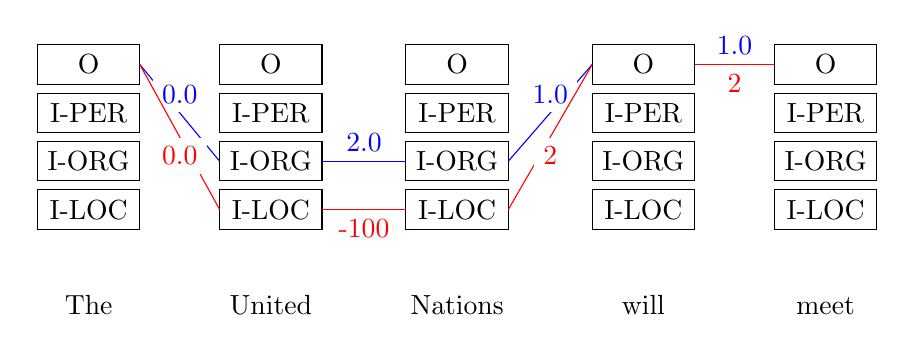
\begin{tikzpicture}
    \LatticeB
    \draw[blue] (network-1-1.east) -- node[above,fill=white]{0.0}  (network-3-2.west);
    \draw[blue] (network-3-2.east) -- node[above,fill=white]{2.0} (network-3-3.west);
    \draw[blue] (network-3-3.east) -- node[above,fill=white]{1.0} (network-1-4.west);
    \draw[blue] (network-1-4.east) -- node[above,fill=white]{1.0} (network-1-5.west);
    \draw[red] (network-1-1.east) -- node[below,fill=white]{0.0}  (network-4-2.west);
    \draw[red] (network-4-2.east) -- node[below,fill=white]{-100}  (network-4-3.west);
    \draw[red] (network-4-3.east) -- node[below,fill=white]{2}  (network-1-4.west);
    \draw[red] (network-1-4.east) --node[below,fill=white]{2}  (network-1-5.west);
  \end{tikzpicture}
  \begin{itemize}

  \end{itemize}
\end{frame}



\begin{frame}{Model Choices}
  Discriminative, Markov Models
  \air 

  \begin{center}
    \begin{tabular}{llcc}
      \toprule
      Normalization && Local & Global \\ 
      \midrule
      Linear && MEMM &  CRF \\ 
      Non-Linear && NN-MM &  NN-CRF \\ 
      \bottomrule
    \end{tabular}
  \end{center}
\end{frame}

% \begin{frame}
  
% \end{frame}

%  \begin{frame}{Neural Network-CRF}
   
%  \end{frame}

 % \section{Generative Models with Global Normalization}

 % \begin{frame}
   
 % \end{frame}

\end{document}